\section{Experimentación}
	A continuación, se presentan los cuatro experimentos que se realizaron. Todas las instancias de experimentación se ejecutaron 20 veces, calculando luego el promedio de los valores obtenidos. Con el código del trabajo práctico se incluye una serie de scripts de \emph{bash} que permiten recrear los experimentos realizados, como así también los gráficos que se incluyen en este informe; esto puede hacerse ingresando al directorio \texttt{exp} dentro de la raíz, y ejecutando el comando \texttt{./exp -n 20}.

	\subsection{Experimento 1}
		En el primer experimento se genera una serie de imágenes de diferentes tamaños, tomando una imagen grande y disminuyendo progresivamente sus dimensiones.
		Luego, se ejecuta el filtro \emph{blur} con cada una de las imágenes generadas y se compara el tiempo de ejecución de las implementaciones en C y lenguaje ensamblador.
		Esto se repite para el filtro \emph{diff}, con la diferencia de que para cada tamaño de imagen se genera 
		un par de imágenes con ciertas diferencias entre ellas, para poder verificar el buen funcionamiento del mismo.

		\subsubsection*{Hipótesis} 
			Se espera observar que la implementación en lenguaje ensamblador de ambos filtros sea más eficiente, independientemente del tamaño de la imagen. Esto se debe a que hacen uso del modelo \acr{SIMD}, con todas las ventajas ya mencionadas que esto tiene sobre el rendimiento del código, a diferencia de las implementaciones de los algoritmos en C, que procesan cada píxel de manera independiente. Esto último puede inferirse no solo de la estructura propia del código, cuyos ciclos iteran sobre un único píxel a la vez, sino también de la ausencia de instrucciones \acr{SEE} para procesamiento de valores empaquetados que se observa al desensamblar los objetos obtenidos a partir de este código.

		\subsubsection*{Valores utilizados como parámetros} 		
			En este experimento el ancho de las imágenes utilizadas como parámetro se encuentran en un rango entre 24 y 1800 píxeles.Además, para el filtro \emph{blur} se utilizó $r = 15$ y $\sigma = 5$.

		\subsubsection*{Resultados}
		   	{\centering \begin{tabular}{c}
		      {\small Filtro \emph{diff}} \\
		      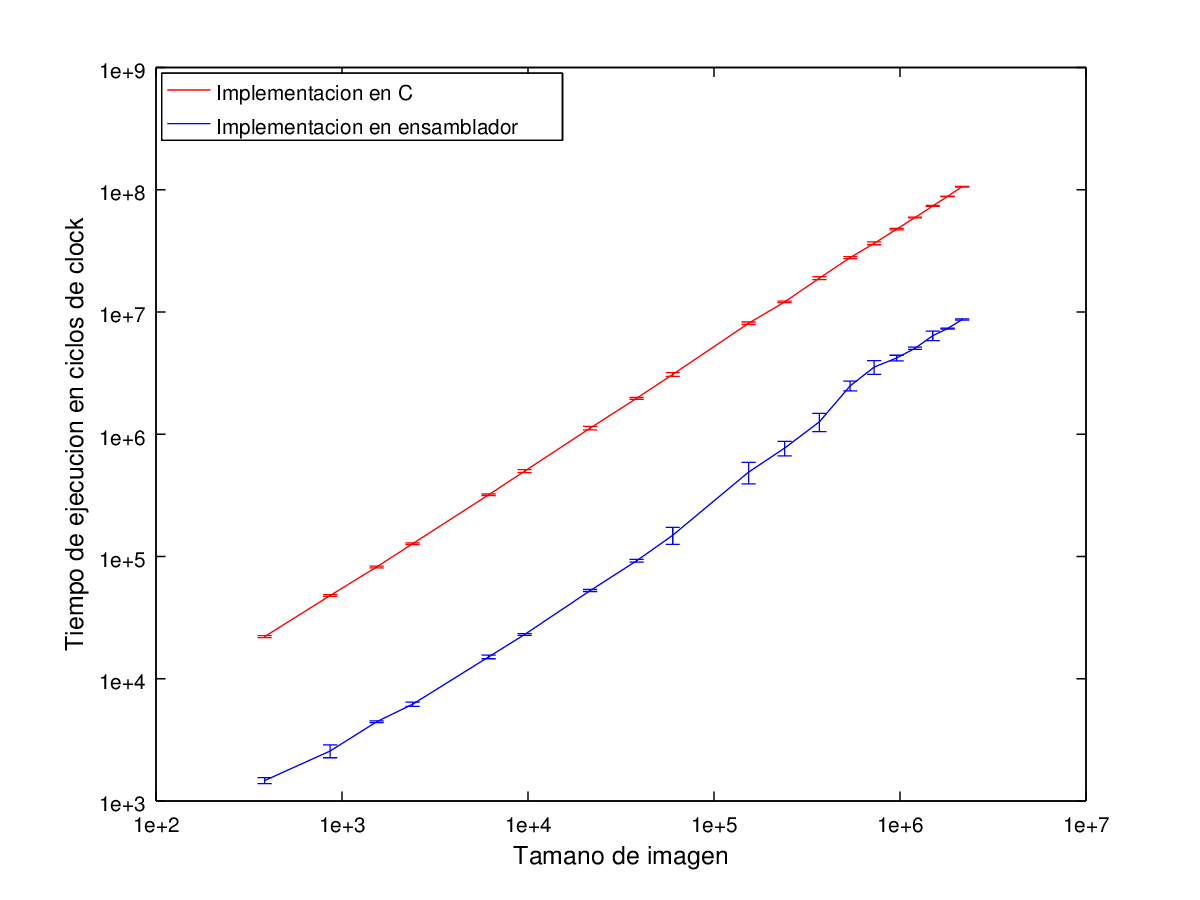
\includegraphics[width=12cm]{../exp/graficos/exp1-diff-c_vs_asm.png} \\
		    \end{tabular}}

		    {\centering \begin{tabular}{c}
		      {\small Filtro \emph{diff} - Tiempo de ejecución normalizado por píxel} \\
		      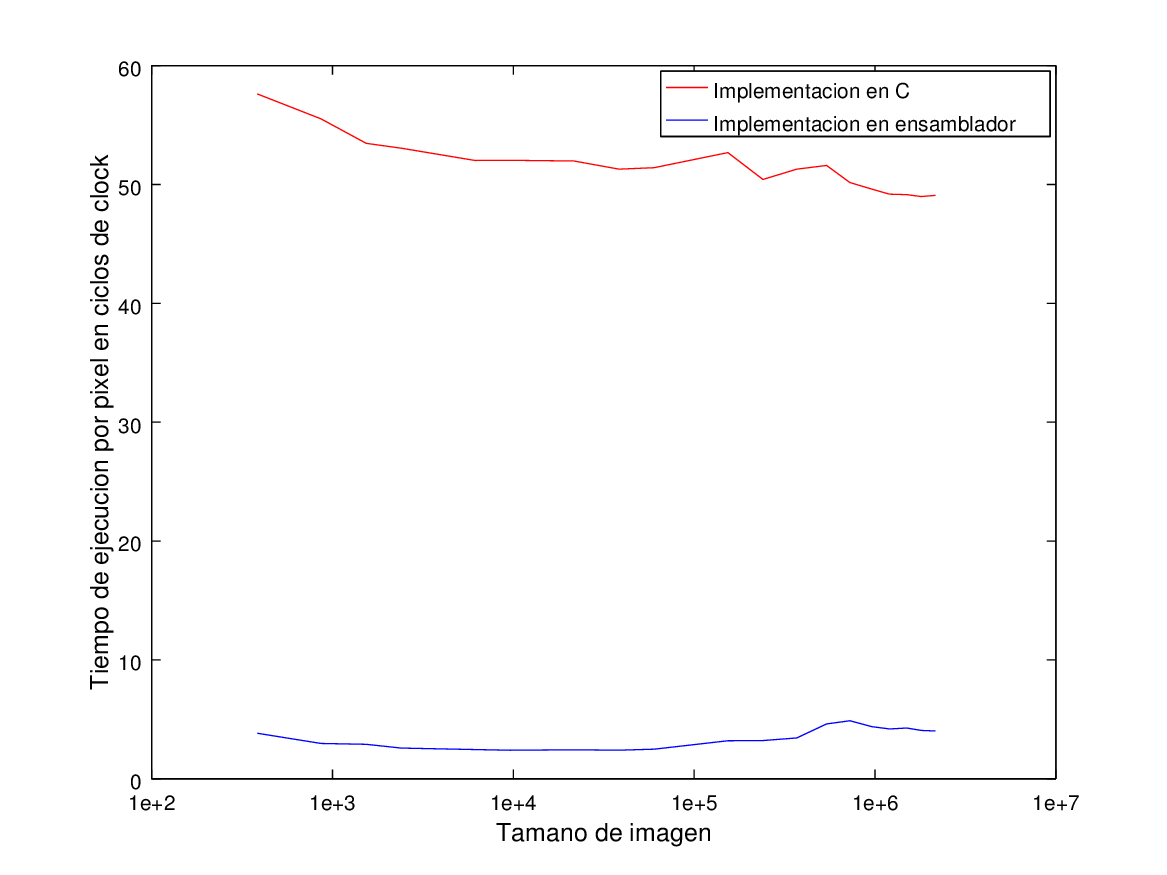
\includegraphics[width=12cm]{../exp/graficos/exp1-diff-tiempo_por_pixel.png} \\
		    \end{tabular}}

			{\centering \begin{tabular}{c}
		      {\small Filtro \emph{blur}} \\
		      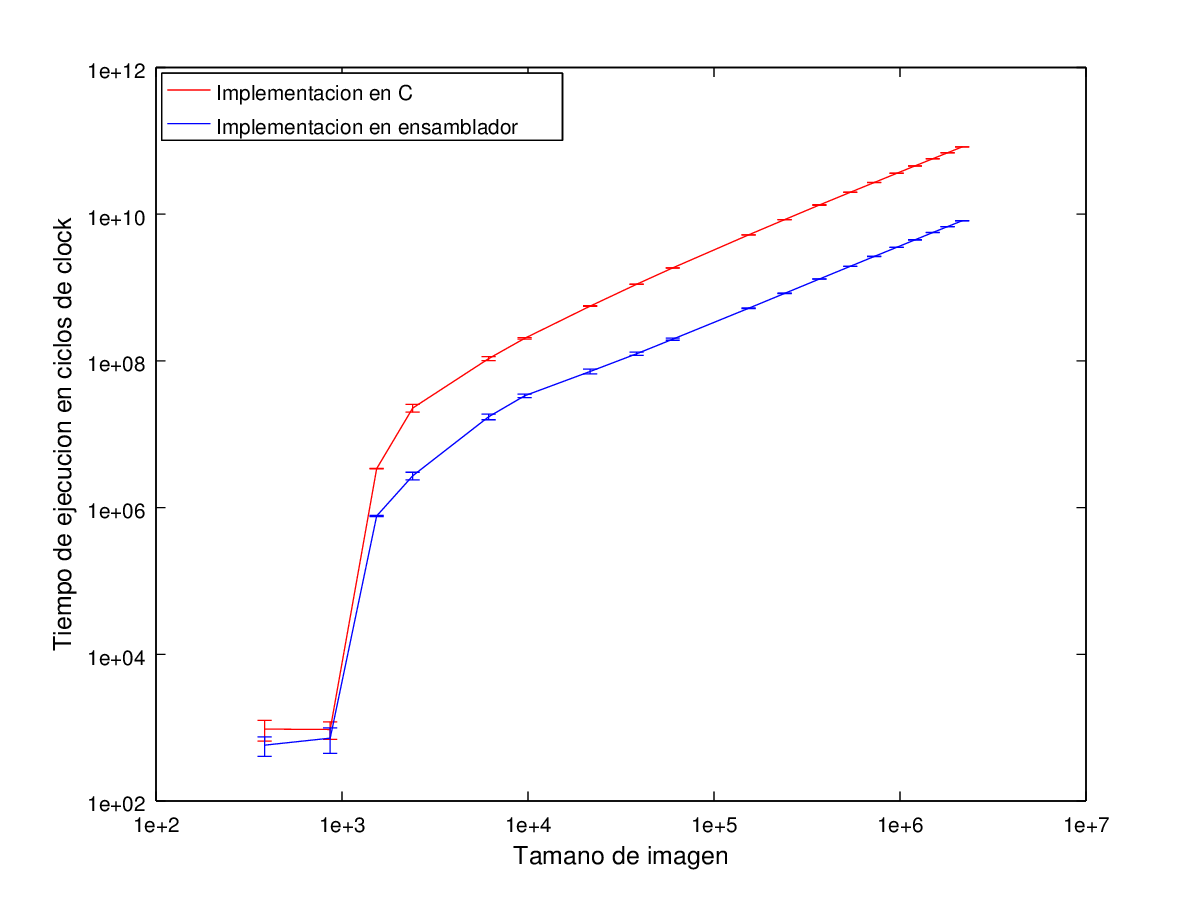
\includegraphics[width=12cm]{../exp/graficos/exp1-blur-c_vs_asm.png} \\
		    \end{tabular}}

		   	{\centering \begin{tabular}{c}
		      {\small Filtro \emph{blur} - Tiempo de ejecución normalizado por píxel} \\
		      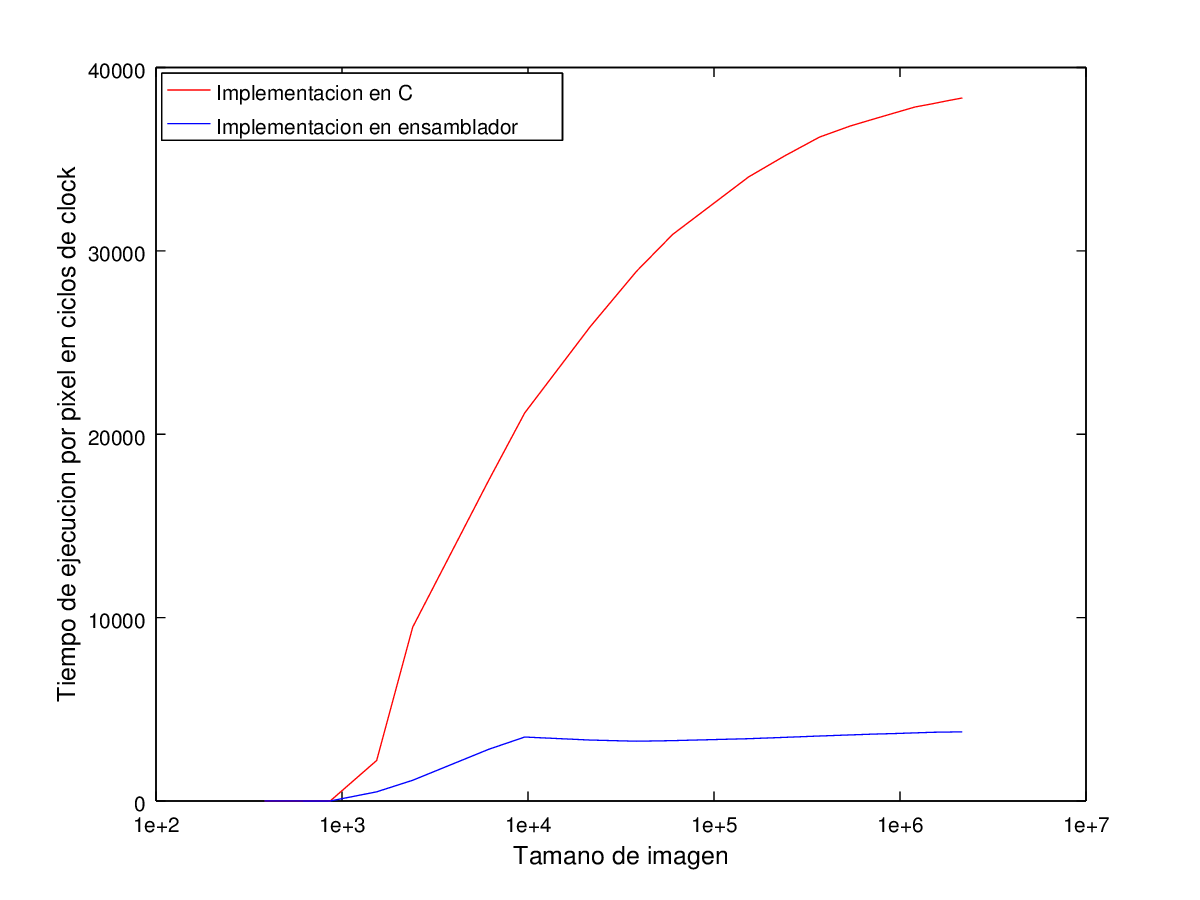
\includegraphics[width=12cm]{../exp/graficos/exp1-blur-tiempo_por_pixel.png} \\
		    \end{tabular}}

		\subsubsection*{Conclusiones y observaciones} 
			Como se observa en los resultados, se pudo confirmar la hipótesis planteada: la implementación en lenguaje ensamblador resultó más rápida que la implementación en C para todos los tamaños de imagen.
			En \emph{blur}, cuando llamamos a la función con un valor de $r$ mayor a la mitad de la altura o a la mitad del ancho de la imagen, no se producen cambios. Dado que en el experimento el valor de $r$ se mantiene constante, las dos imágenes más pequeñas no se ven afectadas por el filtro, lo cual se ve reflejado en los resultados, ya que para estas dos imágenes el tiempo de ejecución es notablemente menor.

	\subsection{Experimento 2}
		El objetivo de este experimento es observar como se ve afectada la eficiencia del algoritmo \emph{blur}, en ambas implementaciones, para diferentes valores del parámetro $r$ manteniendo constante la imagen de entrada.

		\subsubsection*{Hipótesis} 
			Se conjetura que, a medida que el valor del radio $r$ se incrementa, el tiempo de ejecución en las dos implementaciones aumentará, y que lo hará de manera cuadrática con respecto al incremento en $r$. Esto se debe a que la complejidad temporal de cada ejecución del ciclo principal del algoritmo depende del tamaño de la matriz de convolución, que es $(2r + 1) \times (2r + 1) \times 4$, es decir, es cuadrático en el valor de $r$.

		\subsubsection*{Valores utilizados como parámetros} 
		La dimensión de la imagen utilizada es 400 filas y 600 columnas. El valor del sigma es 5 y los radios toman valores entre 1 y 40.

		\subsubsection*{Resultados}

			{\centering \begin{tabular}{c}
	      		{\small Filtro \emph{blur} - Tiempo de ejecución según radio} \\
	      		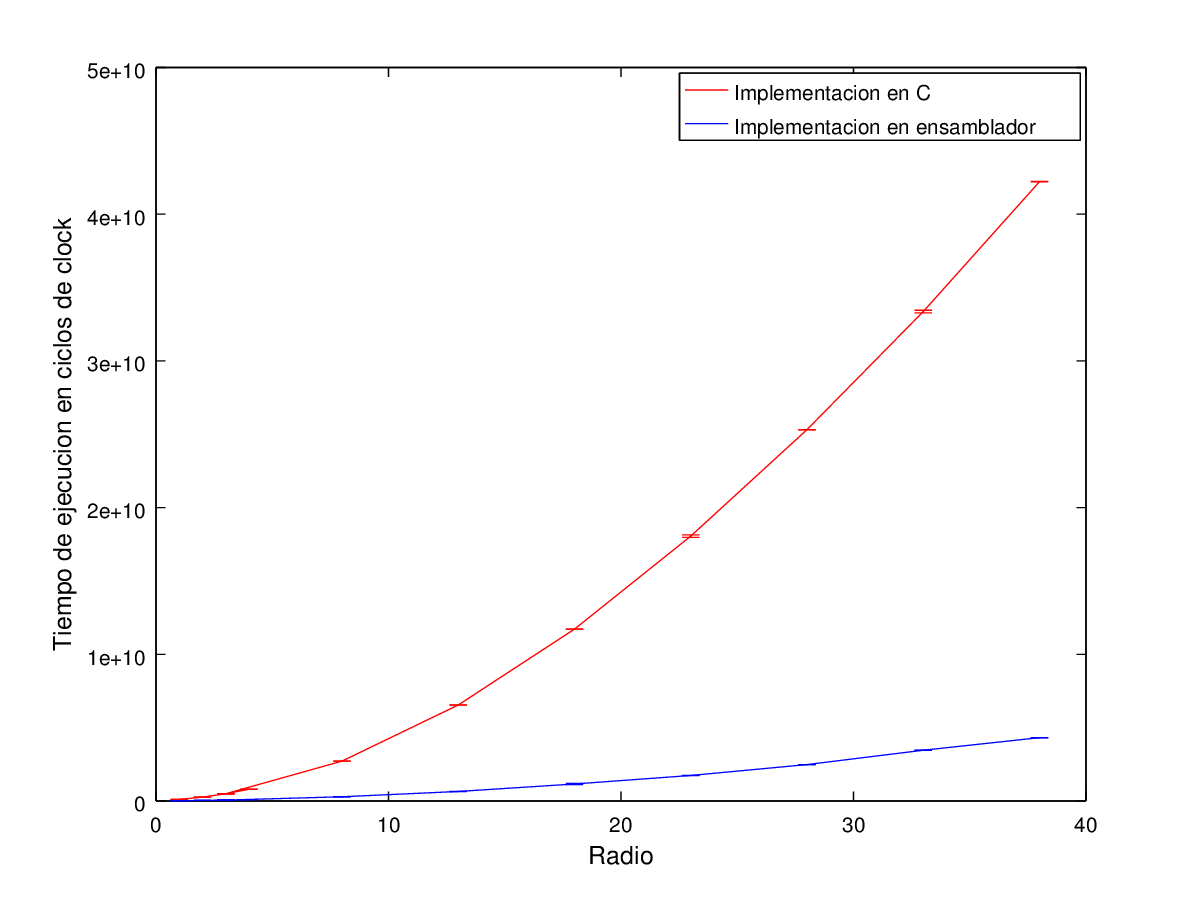
\includegraphics[width=12cm]{../exp/graficos/exp2-tiempo_segun_radio.png} \\
	    	\end{tabular}}

		\subsubsection*{Conclusiones y observaciones}
			Se puede observar en los gráficos que a medida que los $r$ aumenta, también lo hace el tiempo de ejecución. En este sentido, se pudo confirmar la hipótesis. Sin embargo, si se dividen los valores del tiempo de ejecución por su correspondiente $r^2$, se comprueba que la relación no es lineal; es decir, el tiempo de ejecución no varía cuadráticamente con el valor de $r$.


	\subsection{Experimento 3}
		Este experimento es similar al anterior; también se realiza sobre las dos implementaciones del filtro \emph{blur} y se considera siempre la misma imagen. En este caso el valor de $r$ se mantiene constante pero el de $\sigma$ se modifica.

			\subsubsection*{Hipótesis} 
				Debido a que el valor del sigma es utilizado solamente para realizar un cálculo por cada posición de la matriz de convolución, se estima que modificar este valor no alterará el tiempo de ejecución.

			\subsubsection*{Valores utilizados como parámetros} 
				La dimensión de la imagen utilizada es de 400 filas y 600 columnas. El valor del $r$ es 10, y $\sigma$ toma valores entre 0.5 y 50.

			\subsubsection*{Resultados}

			{\centering \begin{tabular}{c}
	      		{\small Filtro \emph{blur} - Tiempo de ejecución según sigma} \\
	      			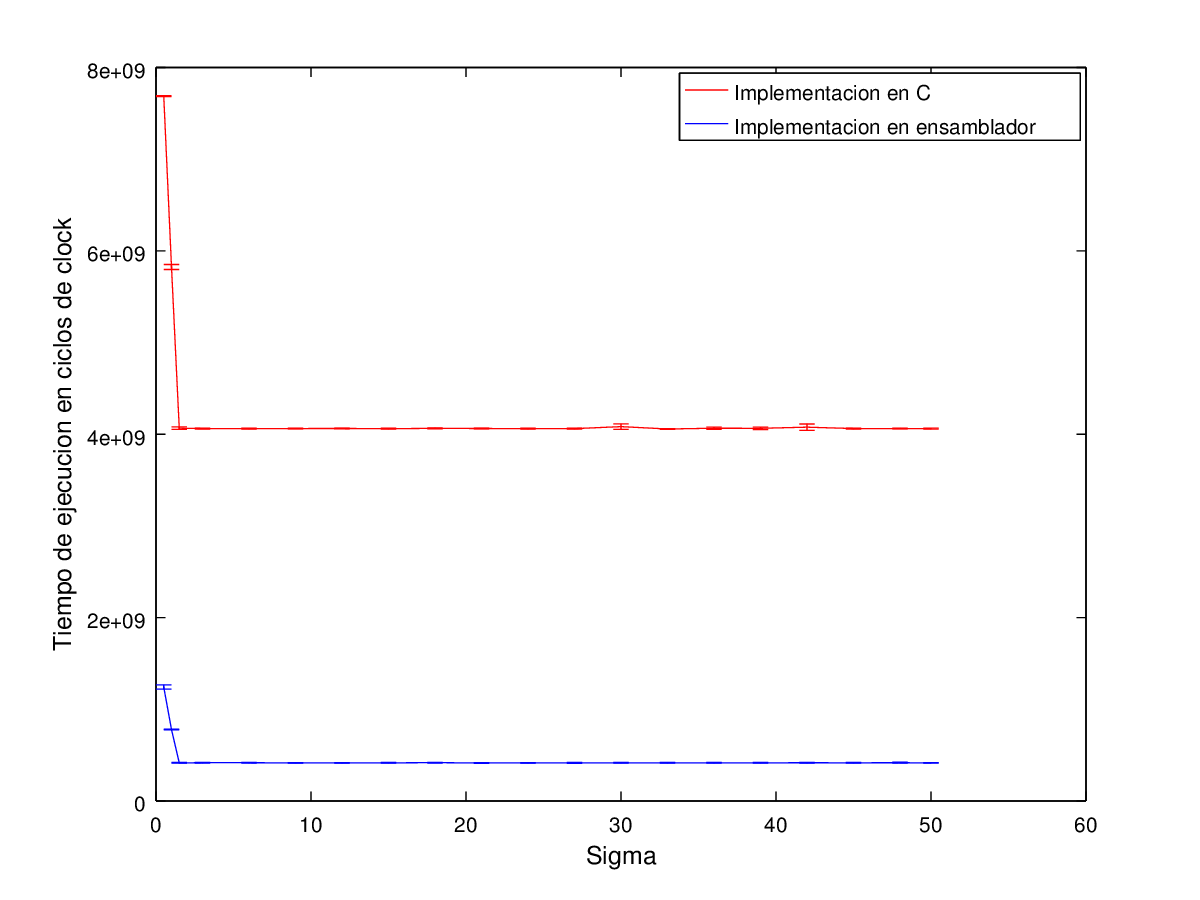
\includegraphics[width=12cm]{../exp/graficos/exp3-tiempo_segun_sigma.png} \\
	    		\end{tabular}}

			\subsubsection*{Conclusiones y observaciones}
				Como se había previsto en la hipótesis, la variación del $\sigma$ no afecta el tiempo de ejecución del algoritmo, tanto en lenguaje ensamblador como en C. Puede observarse que, para valores de $\sigma$ menores que 1, el tiempo de ejecución es notoriamente mayor. Este es un comportamiento inesperado, que sería interesante estudiar posteriormente.

	\subsection{Experimento 4}
		Otras de las pruebas consiste en comparar los tiempos de ejecución de diferentes implementaciones de los filtros en lenguaje ensamblador. Nos interesa medir el peso que tienen en el tiempo de ejecución los llamados a funciones auxiliares. Para esto, queremos comparar el rendimiento de una implementación que utiliza llamados a estas funciones, con el de otra que tiene todas las instrucciones necesarias en el mismo bloque de código (sin utilizar esas funciones auxiliares).
		En particular, se consideraron la versión en lenguaje C de \emph{diff}, a la que se le reemplazaron macros de preprocesador utilizadas para realizar operaciones aritméticas por llamados a función, y la implementación en ensamblador de \emph{blur}, con la que se hizo el proceso opuesto, eliminando los llamados a funciones auxiliares y colocando todo el código directamente en el cuerpo de la función principal.
		
		Este experimento se realiza una determinada cantidad de veces con distintos tamaños de imagen.

			\subsubsection*{Hipótesis} 
				Creemos que la versión del código implementada en lenguaje ensamblador que no realiza llamados a funciones va a tener un mejor rendimiento, ya que se evita el overhead que producen estos llamados.
		
			\subsubsection*{Valores utilizados como parámetros} 
				En este experimento el ancho de las imágenes utilizadas como parámetro se encuentran en un rango entre 24 y 1800 píxeles. Además, para el filtro \emph{blur}, se utilizó $r = 15$ y $\sigma = 5$.

			\subsubsection*{Resultados}
				{\centering \begin{tabular}{c}
		      		{\small Filtro \emph{diff}} \\
		      		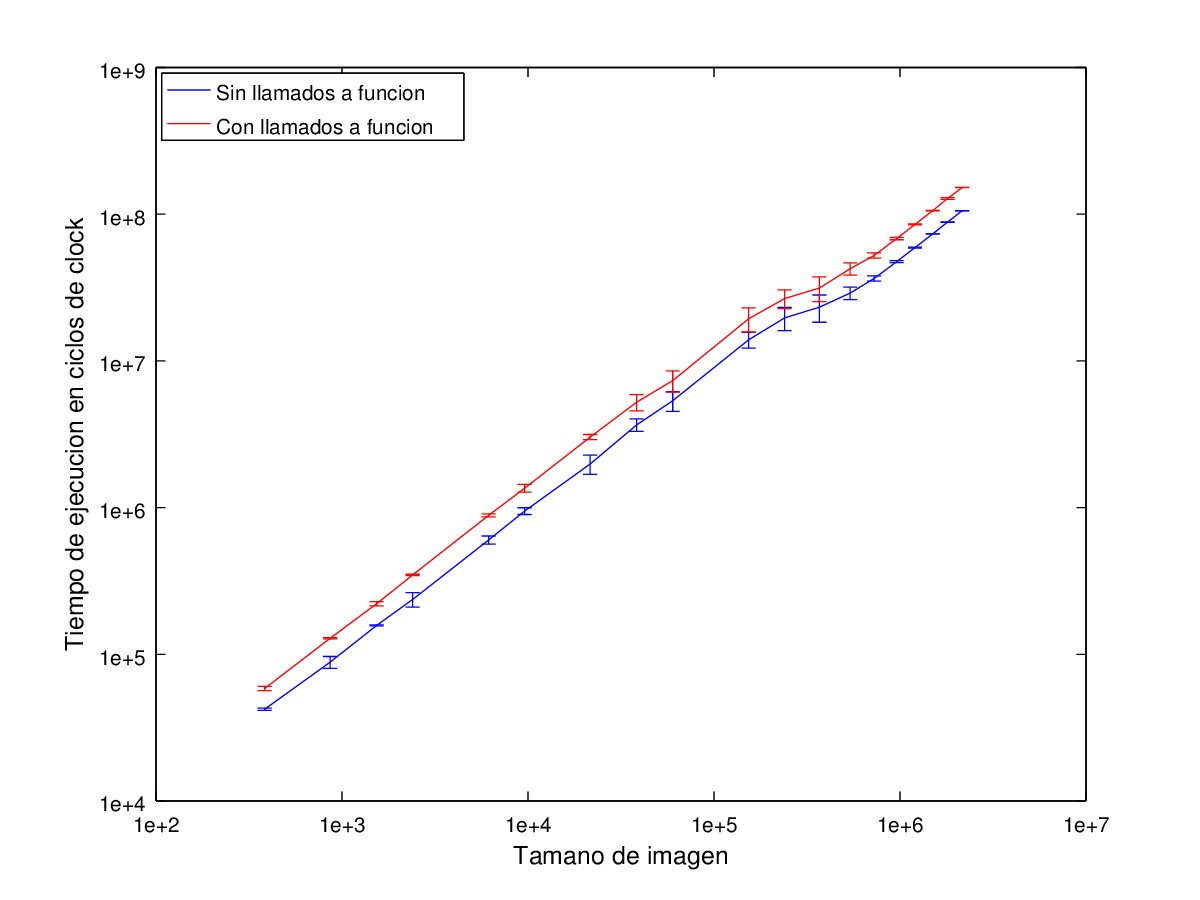
\includegraphics[width=12cm]{../exp/graficos/exp4-diff-c_vs_c2.png} \\
		    	\end{tabular}}

				{\centering \begin{tabular}{c}
		      		{\small Filtro \emph{blur}} \\
		      		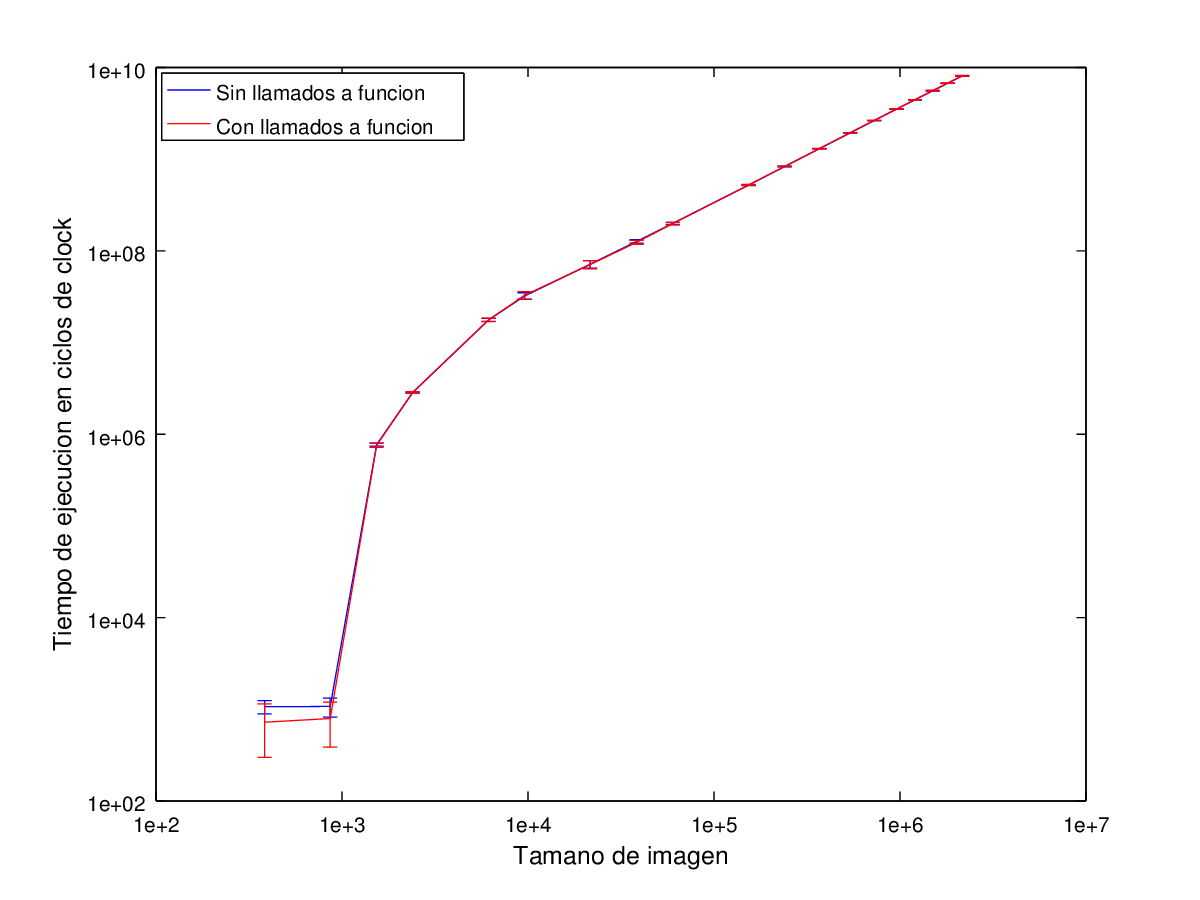
\includegraphics[width=12cm]{../exp/graficos/exp4-blur-asm_vs_asm2.png} \\
		    	\end{tabular}}

			\subsubsection*{Conclusiones y observaciones}		

				Como muestran los gráficos de la implementación en C, los algoritmos que hacen llamados a otras funciones tienen un mayor tiempo de ejecución que las que no los hacen. Esto se debe a que cada vez que se hace un llamado a función, en necesario modificar la pila, manteniéndola alineada y guardando los registros que se deben preservar según la convención C y fueron utilizados a lo largo de la función.

				En lenguaje ensamblador, cuando implementamos el algoritmo sin el llamado a la función auxiliar, sigue siendo necesario acceder a la pila ya que hay que reutilizar registros que se tienen que mantener para la convención C. Por esto, seguimos haciendo accesos a memoria. Una vez que la accedemos es muy posible que en la caché se encuentren los siguientes accesos a realizar. Entonces, la diferencia entre accederla pocas veces o algunas más es muy pequeña, ya que el acceso a memoria caché no es muy caro.

				Posiblemente, si se reformulara por completo la estructura del algoritmo y la manera en que se utilizan los registros, podría lograrse una implementación en lenguaje ensamblador que saque una ventaja más considerable. Sin embargo, esto representaría una labor muy costosa, y hay que tener en cuenta que un código que no realiza llamadas a funciones auxiliares es más difícil de mantener y menos legible, por lo que la ganancia obtenida en rendimiento sería probablemente muy pequeña en relación con las desventajas que se ocasionarían.
